For the remainder, we will focus on distributions of the form 
\[ \pi(x)=\mathcal{Z}^{-1}\e^{-U(x)},\]
where \(\mathcal{Z}\) is a normalising constant. Borrowing some terminology from physics, we call the function \(U:\R^d\to\R\) the potential function. In statistical mechanics, this distribution is known as the Boltzmann distribution. The aim here is to use machinery from physics to solve the problem of sampling accurately. To do this we first must motivate the distribution's origin.

Consider a particle in a potential well of shape \(U\). The equation of motion for such a particle is \cite{Langevin1908}, 
\begin{equation} \dif X_t = -\nabla U(X_t)\dif t +\sqrt{2}\dif W_t. \label{eq:ODLang}.\end{equation}
Here, \(X_t\) is the displacement of the particle from the origin at time \(t\), \(W_t\) is a \(d\)-dimensional Wiener process (Brownian motion) and \(U:\R^d \to \R\) is the potential function. The form of interest here is the \emph{overdamped} Langevin equation, in which the particle experiences no average acceleration, obtained as the high friction limit of full Langevin dynamics.

From the form of the equation, it can be seen that the particle moves down the slope of the well, ``sliding'' towards the minimum energy state. As each particle moves randomly, it is natural to ask what is the average position of many particles in such a well? One would expect the average position to be the one that has lowest energy. To recast the question in statistical language, we ask what is the expected value of the random variable \(X_t\)? This is exactly the goal of MCMC given in Section \ref{sec:intro}. In fact for the Langevin equation, we can give the probability of a particle being at any given displacement. This probability is given exactly by the measure \(\pi\), the Boltzmann distribution. For a diffusion process such as Equation \ref{eq:ODLang} this is called the \emph{stationary distribution}\footnote{Another common term is \emph{invariant measure}}. To show that \(\pi\) is indeed the stationary distribution we use the following lemma.

\begin{lemma}
	For a one-dimensional It\^o diffusion\footnote{That is \(X_t\) solves \(\dif X_t = \mu(X_t)\dif t +\sigma^2(X_t)\dif W_t\)}, suppose \(\sigma^2(t,x)\) is bounded. Suppose that the transition probabilities of \(X_t\) admit a density for every \(t>0\). Further assume that \(\mu(X_t),\sigma^2(X_t) \in C^2\). Define the Fokker-Planck operator, \(\L^*\), as
	\[\L^*:= -\partial_x(\mu(x)\cdot)+\frac{1}{2}\partial^2_x(\sigma^2(x)\cdot).\]
	Then a measure \(\pi\) is invariant for the diffusion if and only if
	\[\L^*\pi = 0\]
\end{lemma}
The proof of this is omitted however it can be seen by forming the Fokker-Planck equation for the probability density of the diffusion. If a diffusion admits a unique stationary measure, then it is ergodic. This fact means one can apply Theorem \eqref{thm:ergodic} and calculate expectations using Langevin dynamics. The proof that \(\pi\) is the stationary measure of Equation \eqref{eq:ODLang} is given only in the one dimensional case, however it is extendable to higher dimensions. For the Langevin equation, the Fokker-Planck operator is

\[\L^* = \partial_x(U'(x)\cdot)+\partial_{xx}\cdot . \]
So it remains to calculate \(\L^*\pi\).
\begin{align*}
\L^*\pi &= \pd{}{x}\bigg\lbrack U'(x)\pi(x) + \pd{}{x}\pi(x)\bigg\rbrack\\
		&= \pd{}{x}\bigg\lbrack U'(x)\mathcal{Z}\e^{-U(x)}+ \left(-U'(x)\mathcal{Z}\e^{-U(x)}\right)\bigg\rbrack\\
		&= \pd{}{x}\lbrack 0 \rbrack\\
		&= 0
\end{align*}
Hence \(\pi\) is indeed the invariant measure of \eqref{eq:ODLang}. \qed
\\
\\
Although this shows that the Langevin equation has an invariant measure, the question of convergence to this measure remains unanswered. Roberts and Tweedie give the following restriction \cite{RT96}.
\begin{theorem}[Theorem 2.1, \cite{RT96}]
	Let \(P^t_X(x,A) = \P(X_t\in A | X_0 =x_0)\) and suppose that \(\grad U(x)\) is continuously differentiable and that, for some \(N,a,b < \infty\),
	\[\grad U(x)\cdot x \leq a|x|^2 + b, \qquad |x|>N. \]
	Then the measure \(\pi\) is invariant for the Langevin diffusion \(X\). Moreover, for all \(x \in \R^d \) and Borel sets \(A\),
	\[\|P^t_X(x,\cdot) - \pi \| = \frac{1}{2}\sup_A \big|P^t_X(x,A)-\pi(A)\big| \to 0\]

\end{theorem}

\begin{figure}[ht]
	\centering
		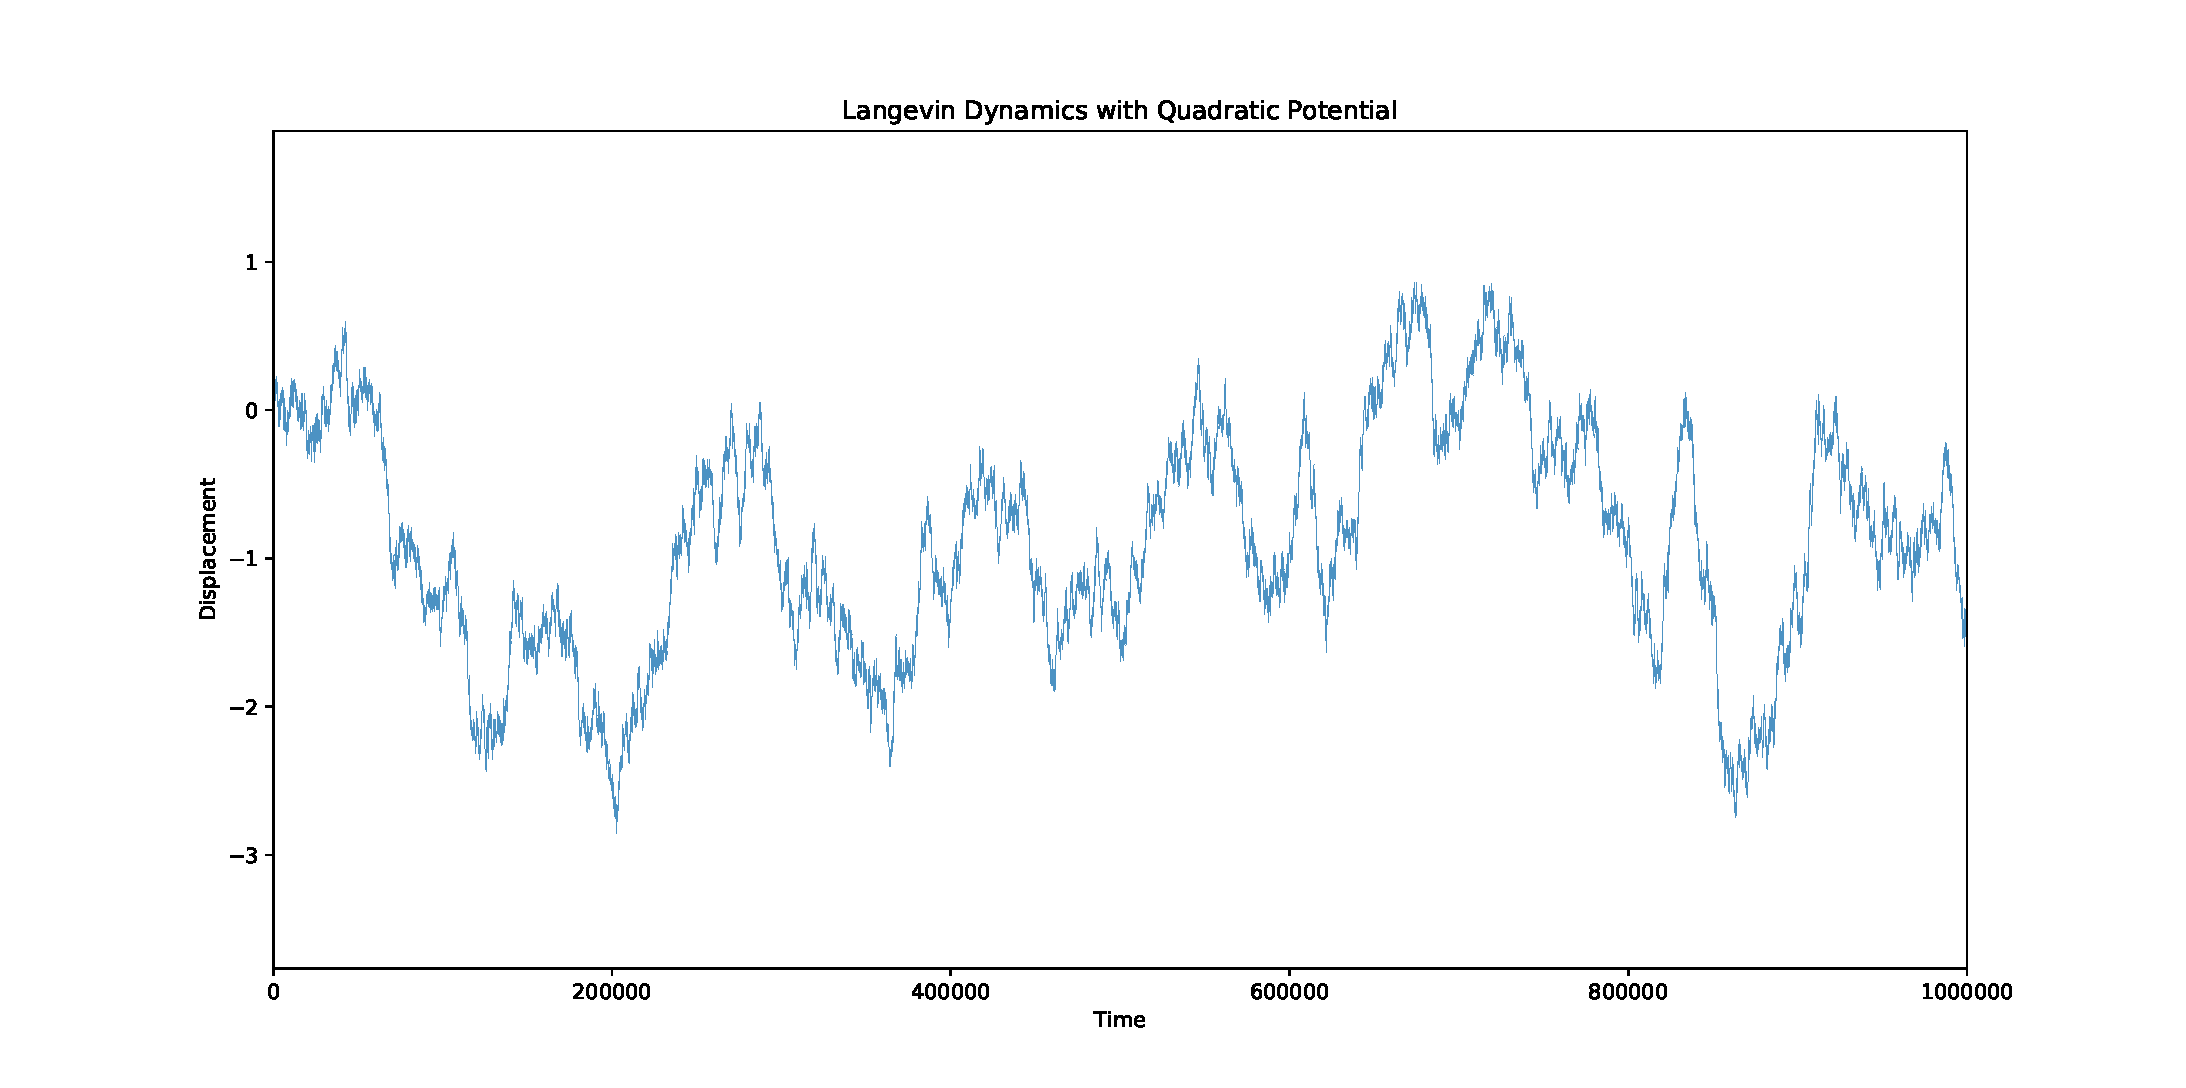
\includegraphics[width=\linewidth]{quadraticLD.pdf}
	\caption{Simulating Langevin dynamics in one dimension with a quadratic potential \(U(x)=x^2/2\)}
	\label{fig:quadLD}
\end{figure}

The problem of sampling from the high dimensional distribution has been reduced to being able to accurately simulate Langevin dynamics. This is not as simple as it sounds. To simulate the continuous process  \eqref{eq:ODLang}, it must first be discretised. Doing so may not preserve the convergence to the invariant measure. The discretised process may not have the same stationary measure or it may not even exist. This means that the method used to discretise must be chosen carefully to ensure good convergence properties. The most natural way to discretise an SDE is to use the stochastic analogue of the (forward) Euler method used on ordinary differential equations, known as the Euler-Maruyama (EM) method. Doing so leads to the Unadjusted Langevin Algorithm (\texttt{ULA}).

\subsection{The Unadjusted Langevin Algorithm}
Applying the Euler-Maruyama method to Equation \eqref{eq:ODLang} gives the following iterative scheme.

\[X_{n+1} = X_n -h \nabla U(X_n) +\sqrt{2h} Z_{n+1},\qquad X_0= x_0 \]
Here the \(Z_n \) are i.i.d. standard normal random variables and \(h\) is the step size. This is equivalent to \(X_{n+1} \sim N(X_n - h\grad U(X_n), 2h I_d )\).\footnote{\(I_d\) denotes the \(d \times d\) identity matrix.} A simple example shows that this discretisation does not converge to \(\pi\). Let \(\pi\) be a standard Gaussian distribution, that is \(U(x) = |x|^2/2 \) and choose \(h = 1\). Then the update is given by

\begin{align*}
	X_{n+1} &\sim N(X_n - \grad U(X_n), 2)\\
	& \sim  N(X_n - X_n, 2)\\
	& \sim N(0,2) \nsim \pi .
\end{align*}
So the chain converges immediately, but to the wrong distribution. Let \(\pi^{\text{ULA}}_{h} \) denote the stationary distribution of \texttt{ULA} with a stepsize \(h\). This is not the only issue that can occur. As well as not converging to the correct distribution, the discretised chain may not be  ergodic, even when the continuous diffusion is exponentially ergodic \cite{RT96}. In particular, the algorithm misbehaves when the gradient of the potential is superlinear. That is,
\[\liminf_{\|x\|\to \infty} \frac{\|\grad U(x)\|}{\|x\|} = +\infty. \]
To mitigate these issues there are two main approaches: taming the gradient and Metropolisation. A further third method involves using a different discretisation scheme.  Our main focus will be the former, although all three approaches will be discussed.

\subsection{Metropolis Adjustment}
Before describing the Metropolis-adjusted Langevin algorithm \texttt{MALA}, it is pertinent at this point to recall the random walk Metropolis-Hastings algorithm \texttt{RWM }\cite{Hastings70, Metropolis53}. This popular variant of the Metropolis-Hastings algorithm \emph{proposes} values and then accepts/rejects them according to some probability \(\alpha\).  So given \(X_n\), propose a candidate \(Y_{n+1}\) as

\[Y_{n+1} = X_n  + \sqrt{2h} Z_{n+1}.\]
Once again, \(h\) is the stepsize and \(Z\) is a normal random variable. Then, accept or reject this proposal using Metropolis rejection, that is with some probability
\[\alpha(X_n,Y_{n+1}) = 1\wedge \frac{\pi(Y_{n+1})q(Y_{n+1},X_n)}{\pi(X_n)q(X_n,Y_{n+1})}.\footnote{Here \(t\wedge s = \min\lbrace t,s\rbrace.\) }\]
Here \(q(x,y)\) is the transition probability, \(\P(Y_{n+1}=y | X_{n}=x)\sim N(X_n, h^2)\). This rejection step is key in creating a kernel that is reversible and thus invariant for the measure \(\pi\). \\


\texttt{MALA} can be seen as another variant of the Metropolis-Hastings algorithm, using Langevin dynamics to propose new states as follows.
\[Y_{n+1} = X_n -h\grad U(X_n) + \sqrt{2h} Z_{n+1}\]
It is perhaps better understood as \texttt{ULA} but with an added Metropolis rejection step \cite{RT96}. Adding this rejection step means the algorithm always has the correct invariant distribution, although convergence is still not guaranteed as the following theorem shows.

\begin{theorem}[Theroem 4.2, \cite{RT96}]
	If \(\pi\) is bounded, and
		\[\liminf_{\|x\|\to \infty} \frac{\|\grad U(x)\|}{\|x\|} > \frac{4}{h}\]
	then the \texttt{MALA} chain is not exponentially ergodic. +++define exp ergodic+++
\end{theorem}
So it can be seen that \texttt{MALA} is not without its issues, and does not solve all the problems of \texttt{ULA}. The concept of taming was introduced to try and reduce the magnitude of these problems.

\subsection{Taming the Gradient}
We have seen that both \texttt{ULA} and \texttt{MALA} run into issues when the gradient of the potential is superlinear. Given an SDE such as \eqref{eq:ODLang}, taming adjusts the drift coefficient in such a way that preserves the invariant measure and improves speed of convergence \cite{Brosse18tULA,RT96,Sabanis13}. To do this, a family of drift functions \((G_h)_{h>0}, \ G_h:\R^d \to \R^d\) are introduced. The SDE to be discretised is thus
	\begin{equation*} \dif X_t = -G_h(X_t)\dif t +\sqrt{2}\dif W_t. \end{equation*}
Applying the Euler-Maruyama method gives the following Markov chain
	\[X_{k+1} =X_k-hG_h(X_k)+\sqrt{2h}Z_{k+1},\qquad  X_0=x_0.\]
To preserve the invariant measure, some restrictions must be placed on \((G_h)_{h>0}\), namely that they are `close' to \(\grad U\) ({\bf A1}) while {\bf A2} ensures ergodicity is preserved and improves stability \cite{Brosse18tULA}. 

\begin{enumerate}[label={\bf A{\arabic*}}]
	\item  For all \(h>0, G_h\) is continuous. There exist \(\alpha\geq 0, C_{\alpha}<+\infty\) such that for all \(h >0 \) and \(x \in \R^d\),
		\[\|G_h(x)-\grad U(x)\| \leq hC_{\alpha}(1+\|x\|^{\alpha}).\]\label{A1}
	\item For all \(h>0\),
		\[ \liminf_{\|x\|\to \infty} \bigg\lbrack \bigg\langle \frac{x}{\|x\|}, G_h(x)\bigg\rangle - \frac{h}{2\|x\|}\|G_h(x)\|^2\bigg\rbrack >0\]\label{A2}
\end{enumerate}
Here we consider two specific taming functions,
 \begin{align*}
 T_h(x) = \frac{\grad U(x)}{1+h\|\grad U(x)\|}, &&  T^{\text{\sc \tiny RT}}_h = \frac{\grad U(x)}{1\vee h\|\grad U(x)\|}.
 \end{align*}
Brosse et al. introduced and studied \(T_h\) whilst Roberts \& Tweedie suggested \(T^{\text{\sc \tiny RT}}_h\), later analysed by Bou-Rabee \& Vanden-Eijnden \cite{BV10MALTA,Brosse18tULA,RT96}. Both taming functions retain the direction of the gradient, only reducing the magnitude of its effect. The latter is the usual \texttt{ULA} until the gradient gets large enough \((\|\grad U(x)\|> 1/h)\), at which point it begins normalising. In contrast, the first will always tame, regardless of size of the gradient. However for the scaling to have noticeable effect, the gradient must be \(\mathcal{O}(h^{-1})\).
When \(T_h\) is the taming function, the algorithm will be referred to as \texttt{tULA}, the tamed unadjusted Langevin algorithm. When the second is applied, it will be called \texttt{MALTA}, the Metropolis adjusted Langevin truncated algorithm after \cite{RT96}. Any tamed algorithm using \(T_h\) will be prefixed with a lowercase \texttt{t}. For a proof that \(T_h\) satisfies \ref{A1} and \ref{A2}, see \cite[Lemma~2]{Brosse18tULA}.
\\
When the problem is ill-conditioned, taming the gradient does not help +++Kostas' example, ill-cond Gauss does this motivate coordinatewise?+++. 
\subsubsection{tULA/c}
So far, the gradient has only been tamed globally. This means that the information the gradient gives is reduced in dimensions where it is not causing divergence. A solution to this is to use coordinatewise taming with the following drift.
  \[T^c_{h}(x) =\left(\frac{\partial_i U(x)}{1+h|\partial_i U(x)|}\right)_{i=\lbrace 1, \dots, d\rbrace} \]
This allows each dimension to be scaled individually. Any algorithm with coordinate-wise taming will be suffixed with a lowercase \texttt{c}.

\subsubsection{Stiff Problems}
To illustrate the effectiveness of coordinatewise taming, consider an ill-conditioned Gaussian distribution with mean \(\mathbf{\mu},\) covariance matrix \(\Sigma\) as follows.
\begin{align*}
    \mathbf{\mu} &= \mathbf{0} && \Sigma = \begin{bmatrix}  \end{bmatrix}
    
\end{align*}
\subsection{Discretise Differently}
An alternative approach is to use a different discretisation of the SDE \eqref{eq:ODLang}, which we consider in this section. The first is an extension of the Euler method \cite{Sabanis18tHOLA}, while the latter uses a non-Markovian scheme developed for use in molecular dynamics \cite{LM12}.
\subsubsection{Higher Order Langevin Algorithm}
As in the ordinary case, the Euler-Maruyama method is not the only way of discretising an SDE. One can also take a higher order expansion, analogous to the Runge-Kutta method in ODE theory, known as the order 1.5 Wagner-Platen expansion\footnote{Or the stochastic Runge-Kutta method \cite{Schaffter10numericalintegration}}. For a one dimensional Langevin diffusion \eqref{eq:ODLang}, this is 
\[X_{n+1} = X_n -hU'(X_n)+\sqrt{2h}Z_n -\sqrt{2} U''(X_n) \tilde{Z}_n +\frac{ h^2 }{2}\bigg\lbrack U'(X_n)U''(X_n)-U'''(X_n)\bigg\rbrack.  \]
Here, \(\tilde{Z}_n\) is defined as
\[  \tilde{Z}_n = \int_{t_n}^{t_{n+1}} \int_{t_n}^s \dif W_r \dif s. \]
This is a Gaussian random variable with mean \(0\) and variance \(\frac{1}{3}h^3 \). Extending this to \(d\)-dimensions and applying to the Langevin SDE \eqref{eq:ODLang} and taming as above gives the following iterative scheme. The untamed version is the same, but with all subscripts removed. {+++ \bf WHERE HAS Z tilde GONE? +++}
\[X_{n+1} = X_n + \mu_{h}(X_n)h +\sigma_{h}(X_n)\sqrt{h}Z_{n+1},\]
where
\[\mu_{h}(x) = -\grad U_{h}(x) +\frac{h}{2}\left( \left( \grad^2U\grad U\right)_{h}(x) - \vec{\Delta}(\grad U)_{h}(x)\right) ,\]
and \(\sigma_{h}(x) = \text{diag}\left(\left( \sigma_{h}^{(k)}(x)\right)_{k\in \lbrace 1,\dots,d\rbrace}\right)\) with,
\[\sigma_{h}^{(k)}(x) = \sqrt{2+\frac{2h^2}{3}\sum_{j=1}^d |\grad^2 U_{h}^{(k,j)}(x)|^2 - 2h \grad^2 U_{h}^{(k,k)}(x)}.\]
The subscript \(h\) indicates a taming of the variable has occurred as follows. For any \(x\in \R^d\),
\begin{align*}
    \grad U_h(x) &=\frac{\grad U(x)}{(1+h^{3/2}|\grad U(x)|^{3/2})^{2/3}}\, , && \grad^2U_h(x) = \frac{\grad^2 U(x)}{1+h|\grad^2 U(x)|} ,\\
    (\grad U\grad^2U)_h(x) =&\frac{\grad^2U(x)\grad U(x)}{1+h|x||\grad^2U(x)||\grad U(x)|}\, , && \vec{\Delta}(\grad U)_h(x) = \frac{\vec{\Delta}(\grad U)(x)}{1+h^{1/2}|x||\vec{\Delta}(\grad U)(x)|}.
\end{align*}
Like in the classical case, the aim here is to improve the rate of convergence by using a more accurate discretisation of the underlying diffusion.

\subsubsection{Leimkuhler-Matthews Method}
The Leimkuhler-Matthews method was developed in \cite{LM12} and cleverly exploits the link between the sampling problem and molecular dynamics. The scheme they developed is as follows:

\begin{equation} X_{n+1} = X_n - h \grad U (X_n) +\sqrt{\frac{h}{2}} (Z_n+Z_{n+1}) \label{eq:LM} \end{equation}

Note that this method is non-Markovian as it incorporates the noise term from the previous iteration. At first glance it appears that this is almost identical to the standard EM scheme, however the slight modification drastically improves convergence.  It is derived by considering both positions and momenta in Langevin dynamics (as opposed to the overdamped equation we have considered thus far which neglects momenta).

\begin{align} \dif X_t = P_t \dif t && \dif P_t = \lbrack -\grad U(X_t) - \gamma P_t \rbrack \dif t + \sqrt{2} \dif W_t \label{eq:LMLang} \end{align}

Here, \(\gamma\) is the friction coefficient. It does no appear in the overdamped Langevin equation as it is the high friction limit of the above system.  Equation \eqref{eq:LMLang} can be seen as a combination of an Ornstein-Uhlenbeck process and Hamiltonian dynamics. Splitting the system in this way allows the exact solution of each part in each time step.

\[ \dif \begin{bmatrix} X_t\\P_t \end{bmatrix} = \underbrace{\begin{bmatrix} P_t \\ 0 \end{bmatrix}} \dif t + \underbrace{\begin{bmatrix}  0\\-\grad U \end{bmatrix}} \dif t + \underbrace{\begin{bmatrix} 0\\ -\gamma P_t \dif t + \dif W_t \end{bmatrix}} \]

The Hamiltonian dynamics have been split further in to A and B.  As well as solving these sections separately at each time step, it is also possible to do fractions of a time step for each term. If we solve in the order BAOAB, that is, half a time step each of B and A before a full time step of the OU process before solving the rest of A and B, we recover Equation \eqref{eq:LM} upon taking the high friction limit. Despite the dependence of iterates, the noise quickly decorrelates. Let \(R_n = (Z_n+Z_{n+1})/\sqrt{2}\). Then,

\begin{align*}
    \langle R_n,R_n\rangle  &= \frac{1}{2} \left( \langle Z_{n+1},Z_{n+1}\rangle +\langle Z_{n},Z_{n}\rangle\right) =1\\
    \langle R_n,R_n\rangle = \langle Z_n,Z_n\rangle = \frac{1}{2}\\
    \langle R_n,R_{n-k} \rangle &= 0,   \quad k=2,3,\dots 
\end{align*}

{\bf +++ LINK IN TO NEXT SECTION +++ }
\begin{figure}[H]
\centering
  \begin{minipage}[b]{0.49\textwidth}
  \centering
    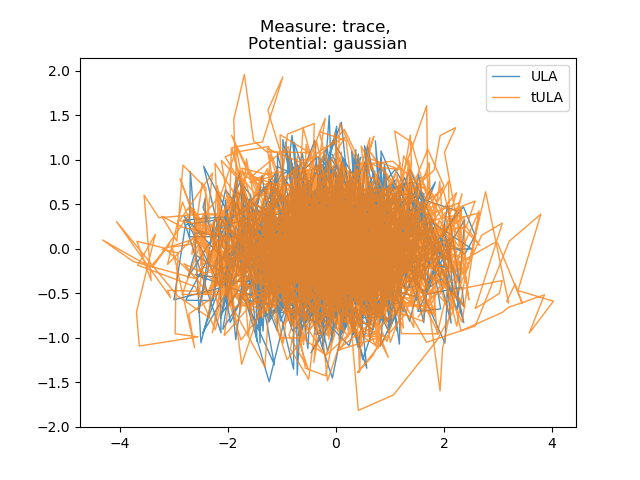
\includegraphics[width=\textwidth]{Figures/ula_tula_step_01.png}
  \end{minipage} %
  \begin{minipage}[b]{0.49\textwidth}
  \centering
    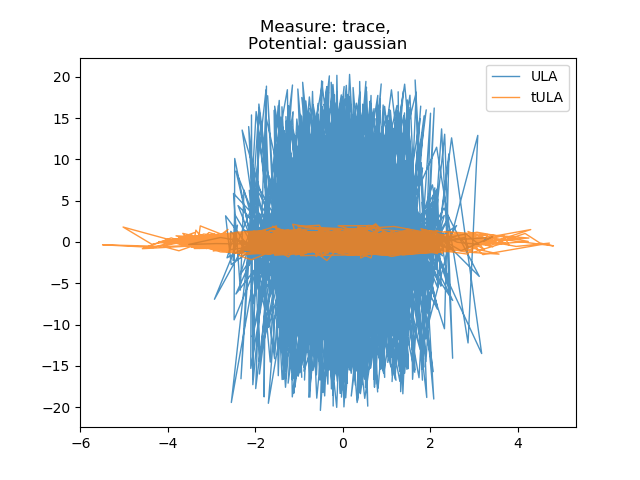
\includegraphics[width=\textwidth]{Figures/ula_tula_step_02.png}
  \end{minipage}
   \caption{\textbf{Demonstration of the stiffness problem with \texttt{ULA}}, resolved by taming. Both \texttt{ULA} and \texttt{tULA} work well for step size $h = 0.1$ on the left, however \texttt{ULA} becomes stiff for a larger step size $h = 0.2$ on the right. For ever higher step sizes, \texttt{ULA} diverges. The distribution here is Gaussian with covariance matrix $\text{diag}(1.0, 0.1)$.}
\end{figure}

\begin{figure}[H]
\centering
  \begin{minipage}[b]{0.49\textwidth}
  \centering
    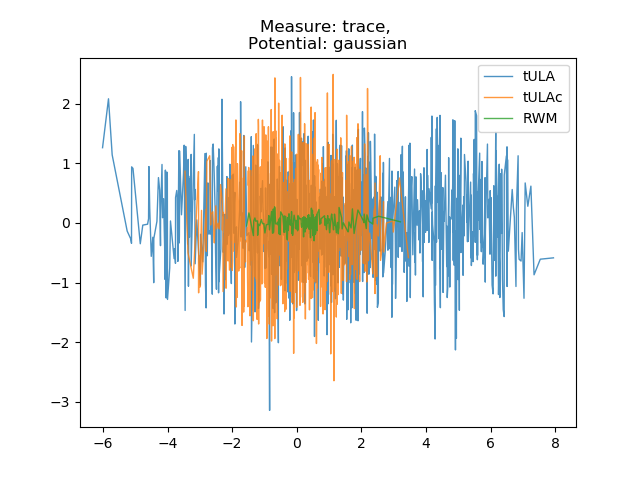
\includegraphics[width=\textwidth]{Figures/tula_tulac_rwm_stiff.png}
  \end{minipage} %
   \caption{\textbf{Coordinate-wise taming} can deal with stiffness in one axis (Ill-conditioned Gaussian distribution with covariance $\text{diag}(1.0, 0.01)$).}
\end{figure}



\begin{figure}[H]
\centering
  \begin{minipage}[b]{0.49\textwidth}
  \centering
    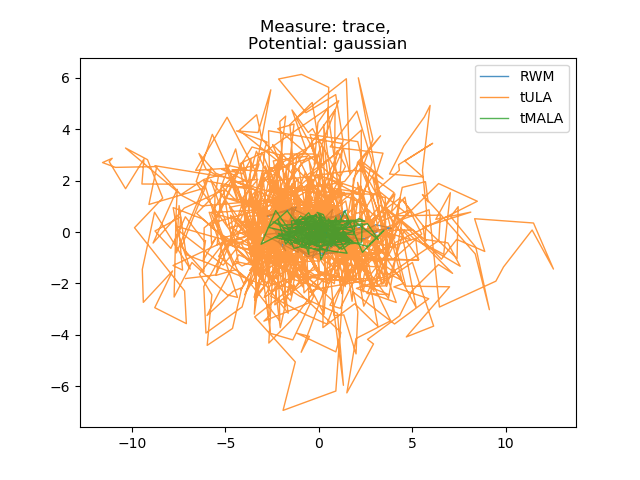
\includegraphics[width=\textwidth]{Figures/tula_tmala_step_1.png}
  \end{minipage} %
  \begin{minipage}[b]{0.49\textwidth}
  \centering
    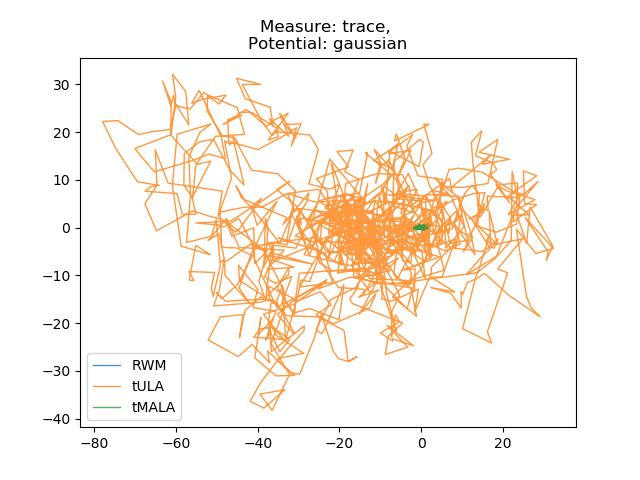
\includegraphics[width=\textwidth]{Figures/tula_tmala_step_10.png}
  \end{minipage}
   \caption{\textbf{Trade-off between rejection-based algorithms and \texttt{tULA} for large step-sizes} ($h = 1$ on the left and $h = 10$ on the right, distribution is Gaussian with covariance matrix $\text{diag}(1.0, 0.1)$). With increasing step size, even \texttt{tULA} starts to suffer from stiffness problems. Rejection-based algorithms resolve the issue, however, their acceptance rate drops very low ($\approx 0.2$ on the left and $\approx 0.03$ on the right). }
\end{figure}




\subsection{Visualization}
A demonstration of the above methods has been implemented using the visualization library of \cite{rogozhnikov2016hmc}\footnote{With kind permission of Alex Rogozhnikov, \url{https://arogozhnikov.github.io/about/}.}. The visualization dynamically follows the trace of a chosen method applied to a chosen two-dimensional distribution. Distributions of various qualitative properties are available. This can be found at the following \textsc{url}: \\
   \centerline{ \url{http://goatleaps.xyz/assets/ULA/ULA.html}}

\begin{figure}[H]
\centering
  \begin{minipage}[b]{0.8\textwidth}
  \centering
    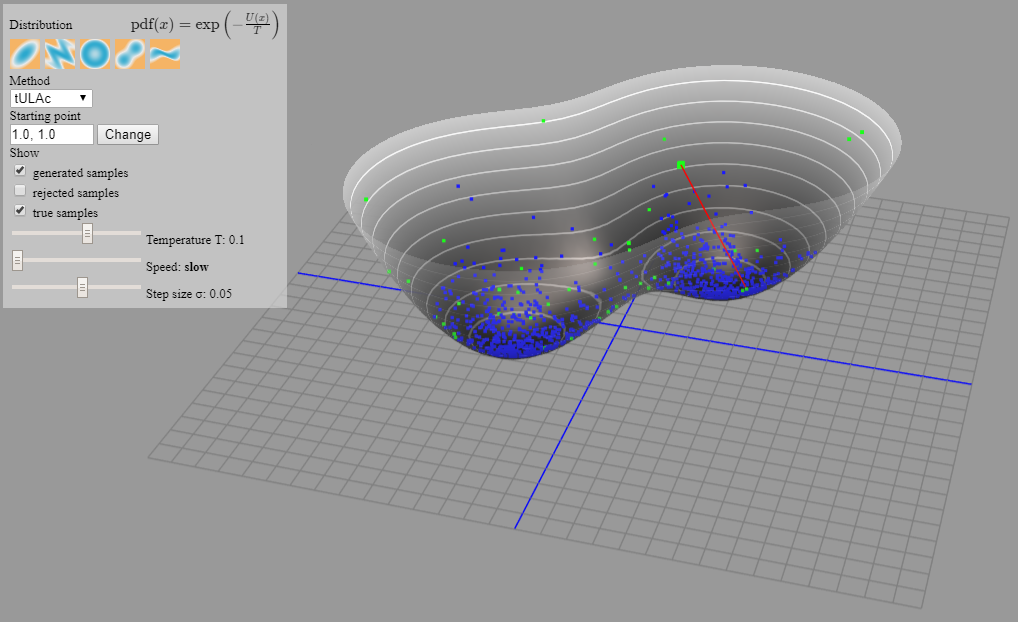
\includegraphics[width=0.8\textwidth]{Figures/ulavis.PNG}
    \caption{Screenshot from the visualization;  tULAc applied to a Gaussian mixture distribution.}
  \end{minipage}
\end{figure}

